\section{Abstract}

Crucial steps for learning a good classification network for the task of HAR in a complex industrial setting will be shown.Ultimately, it can be shown that traditional approaches based on statistical features as well as recent CNN architectures are outperformed.
The design or choice of statistical features is often a difficult process, due to the large intra-class and inter-person variabilities in HAR ~\cite{kreil2016coping}.
intertial measurement units (IMUs)
In three independent evaluation studies the continuous recognition of activity events was investigated and the precision-recall performance analysed.
\section{Introduction}
This work aims to evaluate a wide range of sensory data as well as low cost statistical features to present a list of the most worthy and worthless data on walking activity recognition.

The proposed Approach builds on the idea of having a measure to control the dimensionality of a data set consisting of many variables correlated with each other, by ranking them with a greedy manner.

As it might be expected some activities are easy to distinguish, however distinguishing between walking and walking upstairs is more difficult\cite{randell2000context}.
It appears much more difficult to identify the two stair climbing activities~\cite{kwapisz2011activity}
The contribution of this paper is two-fold:1) 2)

In terms of importance of sensor types in HAR, previous works, such as [][], proved that the accelerometer mostly out performs the gyroscope and as mentioned in [], magnetometer does not provide an effective information in HAR. In this work, we present a more flexible answer to this question and by connecting it to the type of activity and sensor location cover pervious answers.

\section{Related Work}
Maurer et al. [46] applied a Correlation-based Feature Selection (CFS) approach [60], taking advantage of the fact that this method is built in WEKA [61]. CFS works under the assumption that features should be highly correlated with the given class but uncorrelated with each other.

\section{Study Setup}
In this section, we present our main approach as shown in Figure \ref{secFig1}, such as ~\cite{janidarmian2017comprehensive}, ~\cite{s131217472}, for step type detection. The approach is composed of 6 major steps as follows:
\begin{itemize}
  \item Data Collection: In this phase, we collect data from walking action using a \textit{Neblina} module. First, we attached the module to the right leg on thigh of two different individuals and asked them to walk. During three different sessions they walked through up stair, down stair, and flat plane. Next, we performed the same operation while the module was attached to the foot of them.
  \item Data Labeling and Segmentation: In this phase, we labeled incoming raw data with 20 columns of sensory data, time stamp, step type, and step cycle number for each session. Next, we partitioned the sessions into frames corresponding to each step.
  \item Feature Extraction: In this phase, we used statistical tools including mean, median, variance, mean absolute deviation, median absolute deviation , standard deviation, and root mean square, as mentioned in Figure \ref{secFig1} in order to filter abnormal data and remove artifacts as well as high frequency noise.

  \item Feature Selection: Per each sensor position, person, and step type, we aimed to pick most important features. For this reason, we employed two methods to find out which features are more statistically significant as well as which columns are weaker in correlation.

      \textbf{- Remove high correlated features:} To remove highly correlated features, first, we used hierarchical correlation method to characterize similarity among features, next, we considered a threshold equal to 0.5 and removed those features which were correlated more than threshold. Addition to this, in order to detect redundant features, we employed flexible parametric additive model to determine how well each feature can be predicted by other features.

      \textbf{-Remove less statistical significant features:} To detect statistical less significant features, first, we used Bayesian generalized linear model to train a model. Next, we extracted the coefficients with value less than 0.5.

  \item Build Model: After extracting most valuable features, we trained machine learning models using algorithms including linear and neural network through our different data sets.

  \item Evaluate Performance: Our evaluations for each model composed of cross validation and prediction as well as general measurements such as R2, accuracy, precision and F-measure.
\end{itemize}
\begin{figure*}
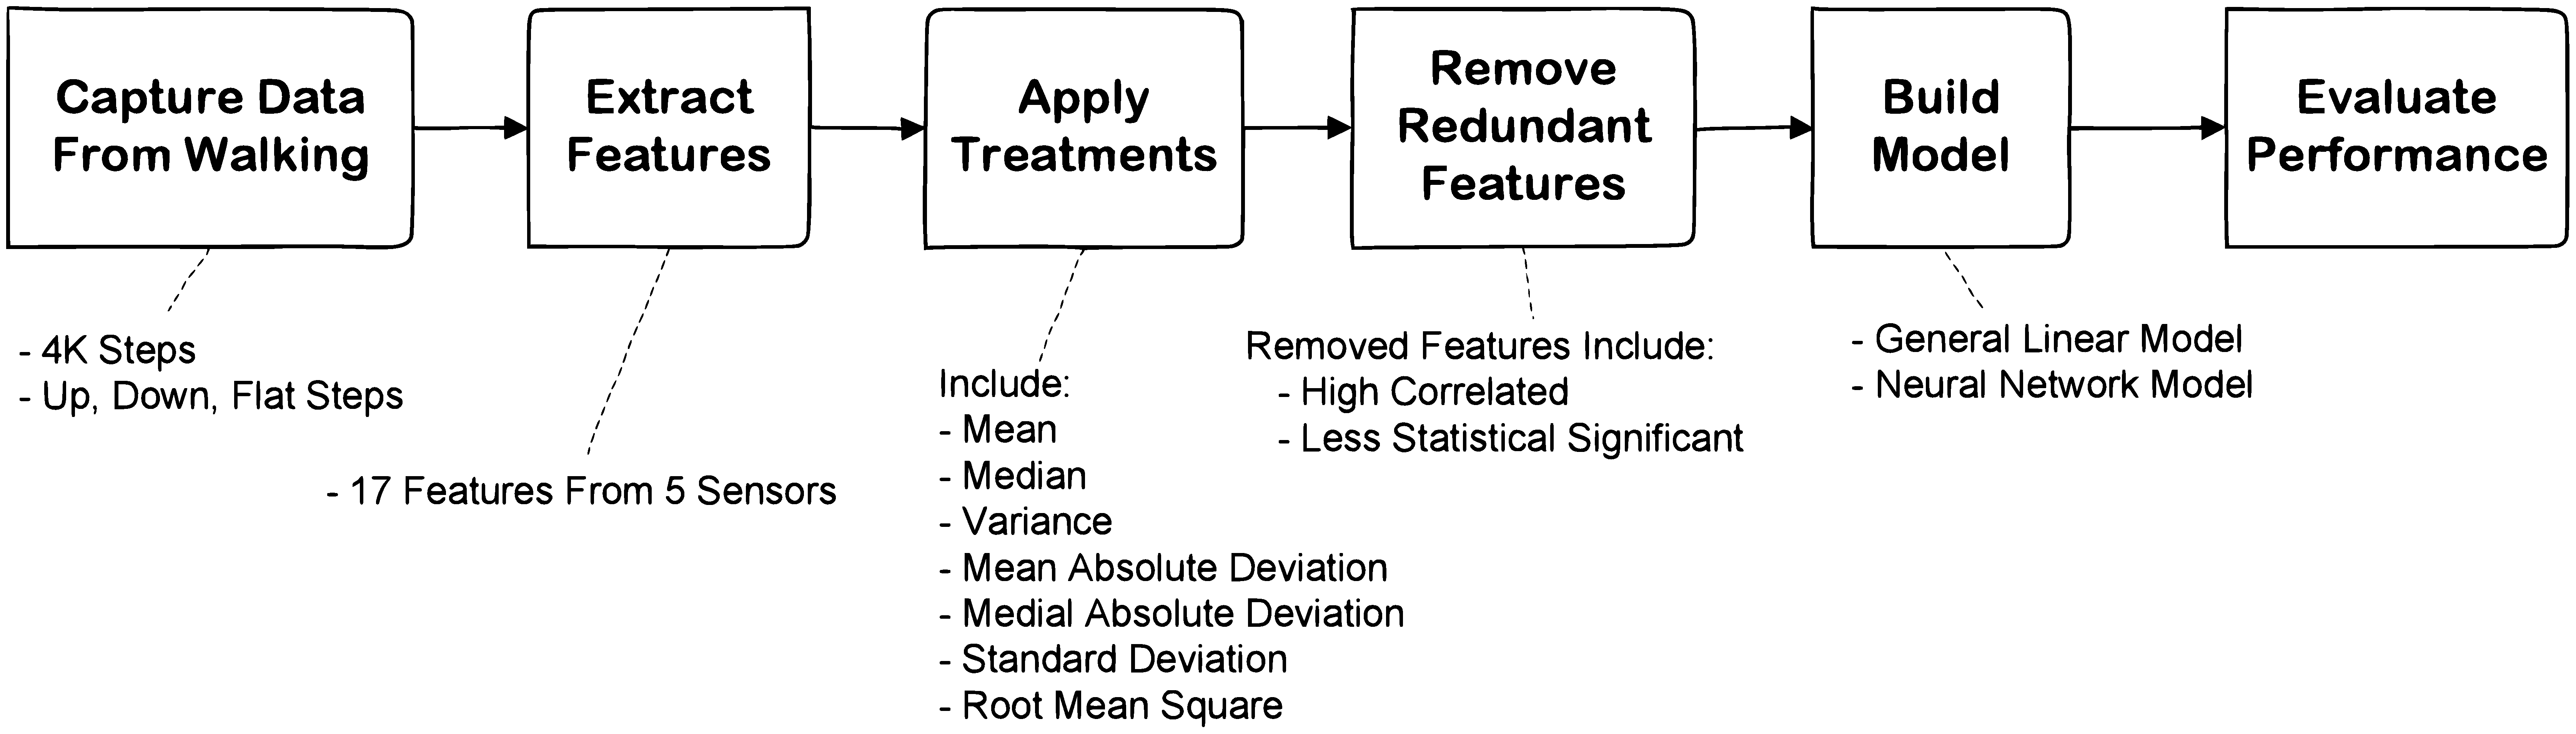
\includegraphics[height=2in, width=6.6in]{approach.eps}
\caption{Step type detection main approach}
\label{secFig1}
\end{figure*}

\section{Data Collection}

In data collection phase, we focused on walking actions as a general daily activities as well as a common action in almost related works. the Walking contains walking on flat floor, ascending stairs and descending stairs.  We prepared two similar experiments with two participants. Both participants were Male, between the ages of 25 and 30 same as the similar work in ~\cite{s140610146}. Attaching sensor to the thigh and foot respectively, each participant performs two trials for each step type at various indoor and outdoor locations without supervision, same as ~\cite{zhang2011feature}. Also, they were encouraged to perform walking activity at their own pace and convenience~\cite{yong2013human}.(needing more details about environment! e.g., how many steps in each experiment-how many stairs,or this:The experimental setup consisted of 10 consecutive trials for SA, DS and W. SA and DS were performed on a staircase composed of four steps and a platform at the upper end, while W was performed on a treadmill.). In each experiment, only one sensor was attached to the participants. The sensor was strapped by an elastic belt on the front of right thigh.  Two sensor positions are shown in Figure \ref{senPosition}. Attaching sensor to either thigh or foot is commonly used in walking detection ~\cite{CAV:CAV2}. We performed study on two positions, two persons and three activities in order to evaluate the effect of different condition on feature redundancy~\cite{zhang2011feature} and the performance of the model, accordingly. The sensors were fixed by a strap to the body of subject. The sampling rate(50 samples per second) is enough to recognize human physical activities ~\cite{6726194}.
For data collection, we employed a module called \textit{Neblina}. The module was equipped with a tri-axial gyroscope, accelerometer, and magnetometer in conjunction with a 32-bit processor\footnote{Specs of version 1} and 2*256KB of flash memory~\cite{ProMotio87:online}.

\begin{figure}
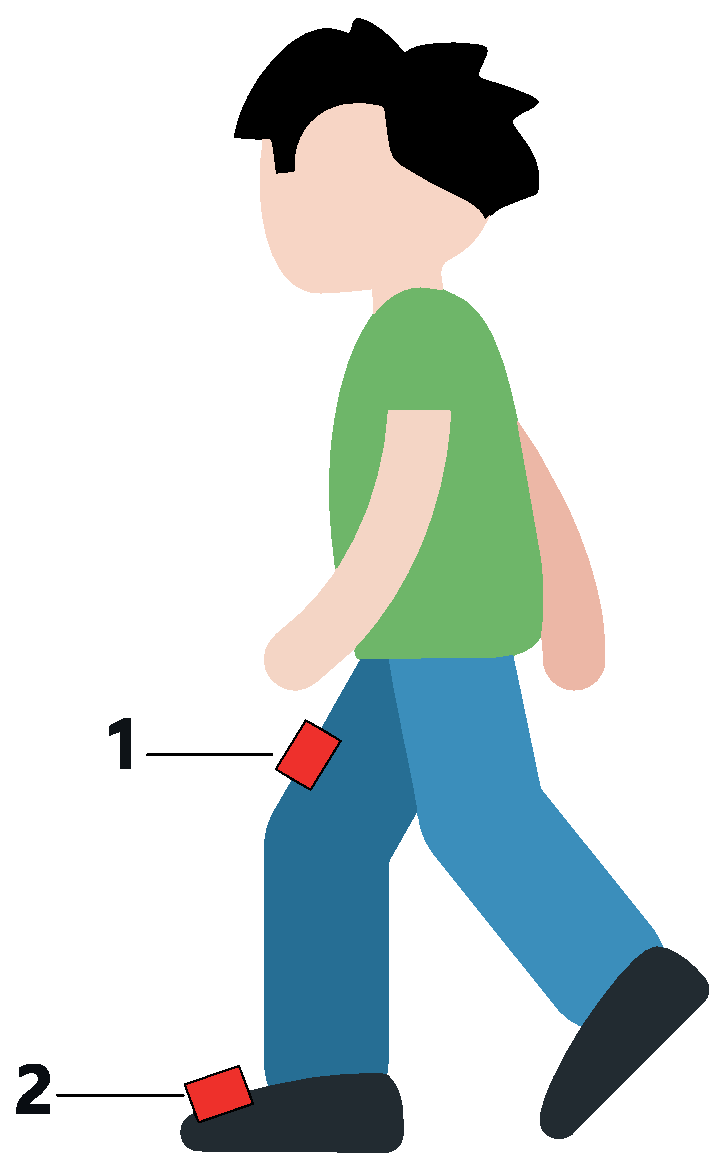
\includegraphics[height=2.0in, width=1.2in]{sensorPosition.eps}
\caption{Overview of the sensor positions on the thigh and foot}
\label{senPosition}
\end{figure}

\subsection{Data}
Data receiving from \textit{Neblina} composes of the following features\footnote{The data available in this address: www.das.conco...}:

\begin{itemize}
\item Acceleration data (ax,ay,az). The acceleration data consists of three columns corresponding with acceleration value of x/y/z axes.
\item Gyroscope data(gx/gy/gz). The rotation values around x/y/z axes are represented in gyroscope columns.
\item Magnetometer data (mx/my/mz). The value of changing magnetic field around the subject in x/y/z axes are stored in these columns.
\item Force data (fx/fy/fz). The force data columns show input force in same direction with acceleration direction.
\item Euler Angle data (yaw/roll1/roll2/pitch1/pitch2). the orientation of the subject which is achieved by composing rotation values about three axes.
\item Time stamp (time). this is the time for recording each sample.
\item Subject id (pid). This column contains an id assigned to each person.
\item Step type (st). This column contains a character corresponding to the type of step.
\end{itemize}


\section{Data Preprocessing}
The collected data from \textit{Neblina} had been stored through several session files which contains the samples of each experiment.
Since the raw data recorded during walking action bring with lots of noise, motion artifacts, and sensor errors, a preprocessing of the data is necessary ~\cite{s131217472}. In this work, because \textit{Neblina} can filter glitches on real-time, there was no need to filter the data any more. So, all actions at this step are as follows:

\textbf{-Trimming data:} we manually deleted the samples which were not applicable to the walking activity from start and end of each 'session'.

\textbf{-Segmenting steps:} The authors in ~\cite{wu2012classification} divided the data into small segments using the sliding window approach. In such approaches, selecting a small enough window size which includes sufficient data to have a reasonable activity recognition performance is the matter ~\cite{s140610146}. However, in this work, the clustering of the step segments has been done automatically on \textit{Neblina} based on the magnetometer's z-axis readings. this information is placed in step cycle time column in data set. Then, we used the step cycle time column to divide the session data sets into step data sets.

\subsection{Features Extraction}
Based on sensory data from \textit{Neblina} in each step data set, we had five angular dimensions for Euler angle and three dimensions for every other data types including accelerometer, gyroscope, magnetometer, and force. We applied 7 treatments on each column of step data sets, as shown in third phase in Figure \ref{secFig1}. So, we extracted 17*7=119 features into our primarily feature set. It should be noted that all features have low or medium complexity in terms of computational cost and are suitable for small size of ram and storage in miniaturized devices such as smartphones ~\cite{figo2010preprocessing}. All extracted features used in feature sets are shown in Table \ref{feature_list}.


\begin{figure*}
\includegraphics[height=3.0in]{high-low-correlation.eps}
\caption{Correlation among features. a) RMS and Pitch are highly correlated, so, they do not provide additional information to distinguish activities. b)mean and median have no similar behavior. addition to this, these features are very helpful to distinguish activities(black circles)}
\label{feature_correlation}
\end{figure*}
\begin{table*}
  \caption{Statistical features and brief descriptions}
  \label{feature_list}
  \begin{tabular}{ | c | c | c | }
    \hline
    Feature&Description&Computational Cost\\
    \hline
    Mean &  The DC component (average value) of the signal over a data set & n\\
    \hline
    Median & The middle number over a data set & n\\
    \hline
    Variance & The square of standard deviation & n\\
    \hline
    Standard Deviation & A measure of how spread out numbers are in the data set & n\\
    \hline
    Root Mean Square & The quadratic mean value of the signal over the data set & n\\
    \hline
    Mean Abs. Deviation & The absolute deviations from mean point over the data set & n\\
    \hline
    Median Abs. Deviation & The absolute deviations from median point over the data set & n\\
  \hline
\end{tabular}
\end{table*}

\subsection{Feature Selection}
\begin{figure}
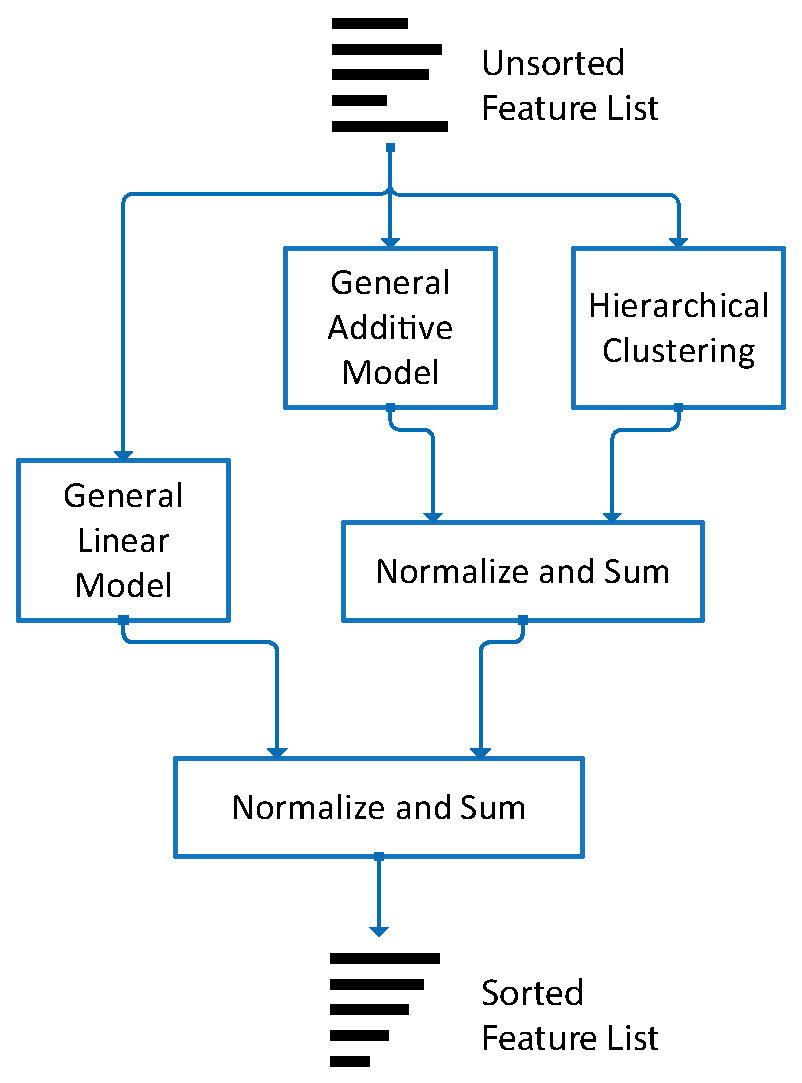
\includegraphics[height=3.0in]{featureSelectionProcess.eps}
\caption{General overview of feature selection process}
\label{feature_selection_process}
\end{figure}
In general, feature selection techniques in classification problems can be grouped into three categories: a)filter methods, b)wrapper methods, and c)embedded methods~\cite{saeys2007review}. The main difference between each category is that how much classification model is involved in selecting features. Filter techniques select features regardless of the model, a common disadvantage of these methods is that they ignore the interaction with the classifier~\cite{saeys2007review}. However, the wrapper methods wraps a selection algorithm around the classification model, thereby keeping a close relation between minimum selected features and best performance in classification. In ~\cite{zhang2011feature}, the wrapper methods has been performed successfully in HAR. On the other side, the overfitting risk and significant computational time are the disadvantages of this method. Comparing with wrapper methods, the embedded methods are one step closer into the classification model. In other word, they are considered as a part of the model, even during testing. Although, the wrapper methods and embedded methods can deliver a better performance rather than filter methods, they can not present the priority among features. Thus, in this work, in order to make a sorted list of features, we employed a method of filter type called 'correlation based feature selection(CFS)'. CFS is a multivariate filter method. We use this method to distinguish a measure to evaluate the importance of features in form of a simple ordered list. For this reason, first, we used a clustering method to measure the correlation of features, which is very important in detecting redundant features. Next, we applied a linear classification model to assess the features in terms of their value to predict each other. If a feature could be predicted by a set of features then it is less important rather a feature with a purely unpredictable behavior. For this step, we used $R^{2}$ measure to evaluate the power of model in prediction a feature. Next, in order to have a statistical evaluation of features, we trained a general linear model and sort descending its terms by absolute value of coefficients. Finally, we merged the sorted lists returned from each step and rank it as a final list. The impact of our sorted list in controlling the accuracy of model is distinguished in discussion part. We performed these steps for every session dataset to have a comparison among activities, sensor positions, and subjects. This sorted feature sets(SFS2-SFS13)is shown respectively from column 1 to 12 in Table[]. The last column(SFS13) is the result of combination of all sessions which will be used in evaluation part. The clustering and classification methods that we used in this section are described in the following:
\begin{figure*}
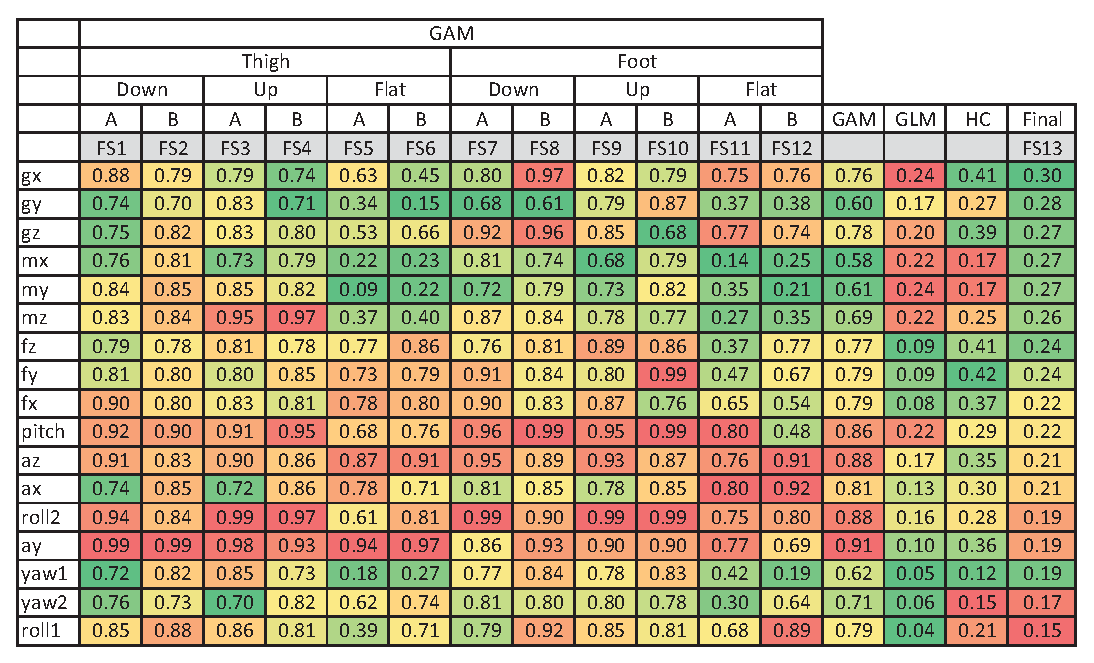
\includegraphics{sensorAxes-sortList.eps}
\caption{List of feature sets}
\label{featureList}
\end{figure*}
\begin{figure*}
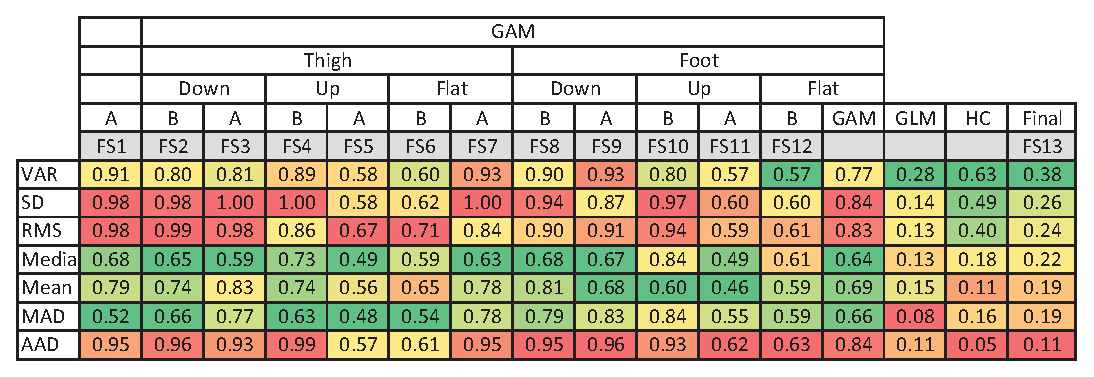
\includegraphics{feature-sortList.eps}
\caption{List of feature sets}
\label{featureList}
\end{figure*}
\subsubsection{Feature Selection Methods}
\begin{figure*}
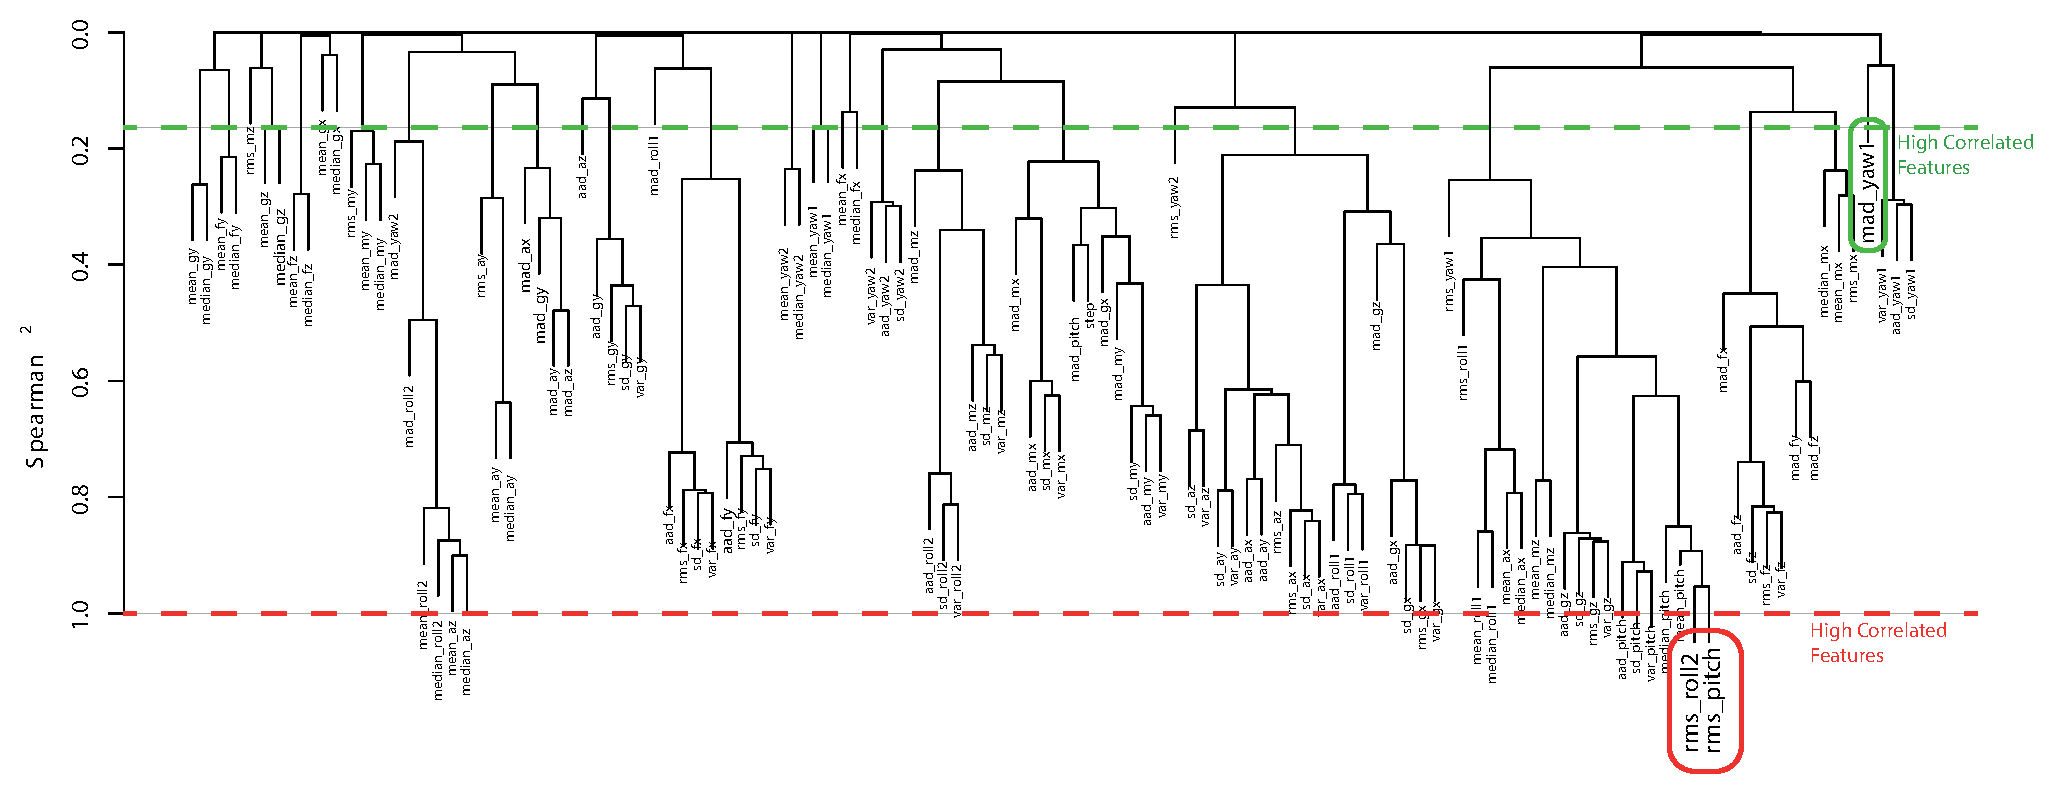
\includegraphics[ width=7.2in]{HirarchicalClustering-treeview.eps}
\caption{A tree view of features in terms of how they are correlated to each other, produced by Agglomerative Hierarchical Clustering method in R }
\label{hierarchical_clustering_diagram}
\end{figure*}
\begin{itemize}
  \item Agglomerative Hierarchical Clustering(AHC)~\cite{WIDM:WIDM1219}:  The similarity measure used in this method was 'squared Spearman correlation coefficients'. Figure [] demonstrate the features and their correlation value in a hierarchical tree view.

   \item Generalized Linear Model(GLM): We trained the GLM because it is popular, simple and it is able to represent the contribution of each feature comparing with others in prediction the response.
        \begin{equation}
        \label{glm_equ}
        Y= b_0 + b_1*X_1+ ... + b_m*X_m
        \end{equation}
Where m is the number of predictors. $X_1$ through $X_m$ represent the m values for the predictor variables and $b_1 \ldots b_m$ are the regression coefficients that represent the independent contributions of each independent variable to the prediction of the dependent variable.

\item Generalized Additive Model(GAM)~\cite{wood2017generalized}: To found out how well each feature can be predicted from remaining features, we used GAM.    
    
       \begin{equation}
        gi(muY)=\sum_{i}(f_{i}(X_{i}))
       \end{equation}
       Where $gi(\ldots)$ is the inverse function of $g(\ldots)$, mu-Y stands for the expected value of Y and  $f_{i}$ is a non-parametric function of the predictor $X_{i}$. Estimating non-parametric functions of the predictor variables, GAM is able to maximize the quality of prediction of a dependent variable Y from various distributions. In this method features are dropped in a stepwise fashion, removing the most predictable variable at each step. Then the left variables provide more important information in prediction. GAM uses $R^{2}$ measurement to evaluate level of accuracy for each step prediction. Table [] provides the features and total their occurrences over sessions measured by this method. Using this method, a range from 20\% through 70\% are considered as redundant through the sessions.
\end{itemize}

\section{Evaluation Approach}

The whole process of data analysis has been performed in R(R Studio). R is a scripting language which provides a wide range of techniques for statistics, visualization and model evaluation. We imported the data from csv files into the R, in form of a \textit{dataframe}(a tightly coupled collections of variables). The name of features is stored in column names while each row represents one step.

In order to evaluate the performance among feature sets we choose two types of validation techniques: 1)\textbf{Cross-person validation} in which the data from one person is used as training and the data from another one for testing. 2)\textbf{Cross-Sensor Position validation} in which we train the model by the data from the sensor located in one position and test it with data from the data of sensor located in other place. Addition to this, since we are curious to measure the impact of having an ordered list of features, we evaluate the accuracy of the model by changing the number of features while picking features starts from top of list against when it is start from end of list.

Besides the influence of different feature sets in performance of prediction, it is interesting to study the effect of different classifiers on identical data set.
Then, We applied two most popular classifiers in the state-of-the-art for activity recognition, linear regression[][][] and neural network[][][], on data set to evaluate them. The classifier, related function and its package are mentioned in Table ~\ref{classification_algorithm}.

\begin{table*}
  \caption{Classification Algorithms}
  \label{classification_algorithm}
  \begin{tabular}{ |c | c | c | c | }
    \hline
    Name&Function&Package&Notation\\
    \hline
    Bayesian generalized linear models &   bayesglm() &arm\{\}& GLM\\
    \hline
    Neural Network &  keras model sequential() &keras\{\}&NN\\
  \hline
\end{tabular}
\end{table*}
\textbf{General Linear Model}
 In this work, we choose Bayesian approach because it offers the flexibility to add data incrementally to allow easy model updating or when a new set of observation arrives~\cite{ramasubramanian2016machine}. Addition to this, Bayesian approach uses a prior distribution (e.g., normal/Gaussian, Poisson, binomial, etc.) to train the model. This distribution will be represented in probable value for coefficients we are attempting to model (e.g., a $b_i$ weight in \ref{glm_equ}). It is important to mention that, the only strong assumption in this method is to make sure the features be purely independent, in other word, any data set violating this property make it performs poorly)~\cite{ramasubramanian2016machine}. As a matter of fact, major inertial sensor signals are highly correlated, So, we enjoy this circumstance of Bayesian approach to evaluate our feature sets with less correlated features.

\textbf{Neural Network}
As the second candidate classifier, we adopt a specified case of neural network. A 5-layer network utilizing two dropout layers (with rates 0.6 and 0.3 respectively) and three dense fully connected layers. Layers use rectified linear (ReLU) activation functions except for a Softmax activation on the one-hot output layer. Similar Network also has been used in ~\cite{O’Shea2016}[] which results efficiently in such cases. We normalized the data using feature scaling to a range from 0 to 1. In our case, dependent variable is a vector with values include 0,.5 and 1 respectively stands for ascending up stair, walking step and descending down stair. To prepare this data for training we one-hot encode the vectors into binary class matrices using the Keras \textit{to\_categorical()} function. We did not use any regularization method, because we prefer to find out the relation among redundant features and performance of model. By the way, it means that our model might be better in terms of generality. so, we left it for future works. More details about layers, output size and the number of parameters are mentioned in Table \ref{nn_model}.
\begin{table*}
  \caption{Neural Network Model}
  \label{nn_model}
  \begin{tabular}{ | c | c | c | }
    \hline
    Layer (type)&Output Shape&Param \#\\
    \hline
    dense\_1 (Dense)&(None, total samples)&features * samples\\
    \hline
    dropout\_1 (Dropout)&(None, total samples)&rate =0.6\\
    \hline
    dense\_2 (Dense)&(None, 100)&12000\\
    \hline
    dropout\_2 (Dropout)&(None, 100)&rate =0.3\\
    \hline
    dense\_3 (Dense)&(None, 10)&1200\\
  \hline
\end{tabular}
\end{table*}
\section{Performance Analysis and Discussion}
In this section, first, we present an appropriate feature set based on sensor type, sensor position and activity type. Next, we compare the predictive power of models in terms of accuracy and generality. Then, after we detect the best feature set and model accordingly, we evaluate the impact of classifier in model performance. We formed these contents into three research questions:

\subsection{RQ1- Which features can detect steps the best?}
In Table [], FS13 represents a sorted list of features based on summation of rank number of each feature in every feature sets(FS1 to FS12). The features with green color closer to the top of list stand for more important features and those are closer to the bottom of list stand for less important. To validate this point, we answer two sub-question: 1)How much it is effective to take feature from top of the list rather than bottom? 2)How much it depends on activity type, sensor position and the subject?

Figure []a illustrates the accuracy of the model over using different number of features during training. To evaluate the impact of an ordered list of features, we trained two model with same classifier but different order of taking features. To train model A, we begin to take feature from top of the list and continuo to take all of them, whereas in model B, the features have been taken from the end of list. As is presented in line-graph for both model, the higher number of features, the better accuracy of model get achieved. However, it is obvious that the model A sharply achieves XX of accuracy using XX features, while model B does not reach the same accuracy even after more XX features. That means, we can save XX number of features only by selecting appropriate set of features. The observations clearly indicate that the ordered feature list has a critical role in terms of decreasing the computational load as well as power consumption in using sensors. Addition to this, it is important to say that this method present a measure to control the accuracy of model only by changing the number of features.

Figure []b specifies the accuracy of models trained on different data sets(rows), varied by 3 activity types, 2 sensor positions and 2 subjects, using different feature sets(columns), FS1 to FS12, which come from respective data sets. Clearly, the feature set corresponding to each data set out performs all other feature sets in terms of power of prediction.
//discuss about figures 

\subsection{RQ2- How much accurately the model can detect steps?}
Since we had located the sensors on two different positions (on thigh and on foot), the objective of this section is to verify the accuracy of models trained on these data sets. Then, we have two models: a) the model trained on thigh sensory data(the sensor located on thigh) including the data from all activity types from both subjects(M\_{t}), b) the model trained on same data type as thigh data set, but from foot sensor(M\_{f}). Both data sets used all available features with the ratio of 70\% for training and 30\% for testing. The GLM classifier had been used for both model. The experiments were performed in the following steps: we trained three models respective to each activity type by using an biased data set contains of 50\% rows of target activity type as target class and 50\% rows equally of two other activity types as the second class. However, during testing, the dataset was unbiased containing equal rows of each activity types. Thus, after each prediction, we compare three responses and define the activity type based on the largest amount. The metrics used were accuracy, f-1, and misclassification. As mentioned in Figure [], the accuracy and f-1 for both sensor positions (thigh and foot) are achieved by 100\%. Compare to the state of art~\cite{janidarmian2017comprehensive}, this approach, considering the sensor fusion, sensor position, segmentation method, and the classifier, is able to achieve a improvement of 4.48\%(among 6 other classifier)on foot model as well as 1.15\%(among seven other classifier) on thigh model.

\subsection{RQ3- How much general are the model?}
The performance of the detection models are adversely affected by cross-dataset evaluation[][][]. This variation get worse with inter person evaluation~\cite{grzeszick2017deep}. To validate this point, we performed two cross-validation approaches (cross-person validation and cross-sensor position validation). In cross-person validation, we tested the model from one subject against the data from another subject separately on data from foot and thigh. In cross-sensor position validation, we tested the model from one sensor position against another sensor position. The results are reported in Table []. Each column contains the amount of accuracy of a specified model(labeled in the caption) over different datasets. Each row represents one dataset. The process of training model and testing is similar to what explained in previous section.

\subsection{RQ4- How much effective is the neural network?}
More recently, approaches based on neural networks (NN) were also picked up to recognize human activity~\cite{lara2013survey}~\cite{kwapisz2011activity}. In those works, NN approaches outperform the traditional approaches, such as Decision Tree or GLM~\cite{kwapisz2011activity}. Nevertheless, it worth to notice that the margin was very narrow and insignificant. To distinguish the performance of NN comparing with GLM, We performed similar experiments with what we did in RQ2 using NN. Technical details about layers have been mentioned in Table \ref{nn_model}. Figure[] compares the results of two classifiers in terms of accuracy, misclassification and F-1.
//discuss about figure

\section{Conclusions and Future Work}
use wrapper methods as a secondary way to improve current method. 